\documentclass[12pt,aspectratio=169]{beamer}
\usetheme{iiasa}

\usepackage{ifthen}
\ifthenelse{\equal{\detokenize{notes}}{\jobname}}{%
\setbeameroption{show only notes}%
}{
%
}

\usepackage[
  maxnames = 1,
  style = authoryear,
  giveninits,
  terseinits,
  maxcitenames = 3,
  ]{biblatex}
\addbibresource{all.bib}
% Small font in bibliography
\renewcommand*\bibfont{\small}
\addbibresource{all.bib}

\usepackage{minted}
\usepackage{pdfpages}

\usepackage{tikz}
\usetikzlibrary{calc}

\title{MESSAGE\emph{ix}-Transport}
\subtitle{Structure, workflow, and applications}
\institute{Energy, Climate, and Environment (ECE) Program \\
  International Institute for Applied Systems Analysis (IIASA)}

\date{
  \texorpdfstring{Message Community Meeting — Wednesday, 29 May 2024}%
  {2024-05-29}}

\author{\texorpdfstring{Paul Natsuo Kishimoto, A. Javaid, T. Hara, V. Krey, B. van Ruijven \scriptsize\newline
  \href{mailto:paul.kishimoto@iiasa.ac.at}%
       {\ttfamily <paul.kishimoto@iiasa.ac.at>}}%
  {Paul Natsuo Kishimoto <paul.kishimoto@iiasa.ac.at>, Aneeque Javaid, Takuya Hara, Volker Krey, Bas van Ruijven}}

\begin{document}

\maketitle

\begin{frame}
\frametitle{Outline}

Briefly introduce MESSAGE\emph{ix}-Transport (MT).

\bigskip
Challenges common to other IAMs and models:
\begin{enumerate}
  \item Applicable for $\gg 1$ project; \structure{reusable} for many research questions.
  \item Integrates with other models/work conducted by a larger team.
  \item Data is scarce and heterogeneous; preparation is expensive.
\end{enumerate}

\bigskip
\structure{Two strategies} used for MT, also usable in similar cases:
\begin{enumerate}
  \item Modularity.
  \item Repeatable workflows.
\end{enumerate}

\end{frame}

\begin{frame}
  \frametitle{Contents}
  \tableofcontents
\end{frame}

\section{MESSAGEix-Transport — goals and structure}

% This frame modified from 2021-12-01 IAMC (Overleaf)
\begin{frame}{What is “MESSAGEix-Transport”?}

A \structure{“variant”} of the MESSAGEix-GLOBIOM (M-G) model \structure{family}:
\begin{itemize}
  \item Not an entirely different model, but a ‘base’ M-G model with substantial modifications.
  \item Transport systems represented \structure{in greater detail} than base M-G.
  \item Other parts—energy supply, land use, trade, etc.—unmodified.
  \item Evolved from the earlier (ca. 2017) model of \textcite{mccollum-2017}.
  \begin{itemize}
    \item Now called “MESSAGE (V)-Transport” to disambiguate.

    “-ix”indicates use of the new MESSAGE\emph{ix} framework.%
    \footnote{\url{https://docs.messageix.org}}
  \end{itemize}
  \item Capable of representing a wide range of current \& future transport modes, technologies, policies, and other phenomena (next slide).
\end{itemize}
\end{frame}

\begin{frame}
\frametitle{Levels of abstraction}
\begin{columns}[b]
\column{0.65\textwidth}
\includegraphics[height=0.8\textheight]{de-weck-roos-magee-f3.1.png}

\column{0.25\textwidth}
M-T is \structure{less abstracted} than base M-G, but does not model, e.g. components of individual transport vehicles, or individual people.

\bigskip
de Weck, Roos, \& Magee (2011), Fig 3.1, p.47.
\end{columns}
\end{frame}

\begin{frame}
\frametitle{Some intended applications}
\begin{description}
  \item [NAVIGATE project] Contrast different approaches (shift/reduce activity; electrify; improve technologies) to decarbonize sectors including ‘demand’ (transport, residential) and industry.
  \item [SSP 2024 update] Implement distinct narratives for each of the 5 SSPs, with close calibration to recent (2020 and later) data, and supply parametrization for the M-G base model.
  \item [EDITS project] Investigate a “High [wellbeing] with Low [energy demand] (HwL)” narrative.
  \item [MESSAGEix-IL] Represent consumer preferences w.r.t. different light duty vehicle (LDV) technologies in the single-country MESSAGEix-Israel model.
  \item [NGFS, others] Reflect detailed transport-sector response to economy-wide climate policies.
\end{description}

\end{frame}

\section{Three challenges}

\begin{frame}
\frametitle{Challenge 1: Many research questions}
These applications entail research questions (RQs) like:
\begin{itemize}
  \item How will lifestyle changes influence energy demand from transport?
  \item How do transport-sector demands for low-carbon energy carriers (electricity, biofuels, synfuels, ‘green’ hydrogen) compete with demands in other sectors under deep decarbonization?
\end{itemize}

\bigskip
Models built from scratch for each of these RQs separately might look very different…but \structure{building new models is expensive} (in time, which $\approx$ money).

\bigskip
We'd rather have \emph{one} tool that is \structure{easily reusable} or extensible for all such applications—yet without being too complicated or unwieldy.
\end{frame}

\begin{frame}
\frametitle{Challenge 2: Integrate with MESSAGEix-GLOBIOM}

Models in the MESSAGEix-GLOBIOM family have certain features:
\begin{itemize}
  \item Temporal scope (2020–2110) and resolution (5- and 10-year periods).
  \item Spatial scope (global) and resolution (R12 node list; maybe others).
  \item Lists of \texttt{commodity} (energy carriers), \texttt{technology}, etc.
\end{itemize}

\bigskip
Available data/knowledge about transport systems may not match these…

\bigskip
…yet we want to \structure{maximize use} of the rich details on energy supply etc. and careful calibration that colleagues have done of base models/scenarios.

\bigskip
Alternate base models for other applications/RQs—like MESSAGEix-IL; MESSAGEix-IN; others—may have different scope and resolution.
\end{frame}

\begin{frame}
\frametitle{Challenge 3: Data}
\begin{itemize}
  \item Few projections for input/techno-economic parameters that cover the temporal scope.

  {\small Example: costs of light duty vehicles (LDVs) and their components (especially: batteries)—projections rarely go beyond 20 years.}

  \item Data quality (by many criteria) varies widely across the spatial scope.
\end{itemize}

\bigskip
Suppose we choose sophisticated method ‘M’ developed using data for geography ‘G1’ (wealthy country with a well-funded statistical agency).

\bigskip
We may find that data is not available for geography ‘G2’ (many low-income countries/regions).
Then we are cornered: we must find, assume, or construct (make up) data for G2.

This is costly, and model results may reflect little besides our assumptions.
\end{frame}

\begin{frame}
\frametitle{Two strategies}

\large

\begin{description}
  \item [Modularity] Break down methods for handling input data and preparing model data to atomic steps.

  → Allows to respond differently to data limitations in different parts of the transport system/existing sources.
  \item [Repeatable workflows] including tools (an “easy button” to build and solve the model) and practices (push the button often).
\end{description}
\end{frame}

\section{Modularity}

\begin{frame}
\frametitle{Modularity}

Break methods (algorithms, steps, processes) down into \structure{atomic steps}.
Methods for:
\begin{itemize}
  \item Handling \structure{input data}—read files, clean, adjust, (dis)aggregate, harmonize, fill, extrapolate, etc.
  \item \structure{Implementing settings or assumptions} for specific scenarios or configuration (e.g. R12 nodes vs. ISR nodes).
  \item Making \structure{exogenous projections}.
  \item Preparing the parameter data used by the core MESSAGE\emph{ix} implementation.
\end{itemize}

\bigskip
Imagine these as a graph (tree, network) of nodes and edges.
\end{frame}

\begin{frame}
\frametitle{Calculations as a graph}
\begin{columns}[T]
\column{0.48\textwidth}
Example 1:

\medskip
{\LARGE $C = A + B$}
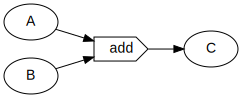
\includegraphics[width=\columnwidth]{genno-ABC.pdf}

\column{0.48\textwidth}
Example 2:
\begin{enumerate}
  \item Load projected GDP for SSP4.
  \item Load projected population.
  \item Compute the ratio of (1) and (2).
  \item Compute index of (3) versus the base-year.
  \item Load historical data on passenger-distance travelled (PDT) per capita.
  \item Project future PDT per capita as a function of (4), (5)
  \item […] (further steps)
\end{enumerate}
\end{columns}
\end{frame}

\begin{frame}
\frametitle{Why do this?}
Instead of “a script” or “a notebook” of 100s or 1000s of lines of code, each \structure{operation} can be described by a simple, short function.
\begin{itemize}
  \item Easily documented, read, and understood.
  \item Easily tested.
  \item Instead of duplicating code, reuse the operator with different inputs.
\end{itemize}

\medskip
Can be implemented using \texttt{genno}, based on \texttt{dask}.
\begin{itemize}
  \item Tracks (very) long chains of calculations.
  \item Same functions/methods can be used \structure{regardless of dimensions, resolution, and units}.
  \item Easy to \structure{graft} different trees on to the graph to swap out methods.
  \item Same framework used for reporting calculations in \texttt{message\_ix} \& co.
\end{itemize}
\end{frame}

\begin{frame}
\frametitle{Dimension \& resolution agnostic}
Recall: $A + B = C$

\bigskip
Dimensionality.
\begin{itemize}
  \item Suppose $A_{xyz} = [ a_{xyz} \in \mathbb{R} ] \quad \forall \quad x, y, z$.
  \item If we choose—say, early in model-building—$B$ can be a scalar $b$.
  \item Later on, we can choose (if we have data, or time to construct detailed assumptions based on a scenario narrative), $B$ can have dimensions like $\{x, z\}$: $B_{xz} = [ b_{xz} ]$.
  \item \structure{Either way}, the code will align with $A$ to produce $C_{xyz}$ with the desired dimensions.
  \item Further calculations on $C$ are independent of whether $B$ was scalar or a matrix.
\end{itemize}
\end{frame}

\begin{frame}
\frametitle{Dimension \& resolution agnostic}
Recall: $A + B = C$

\bigskip
Resolution.
\begin{itemize}
  \item Suppose we change the labels on dimension $z$.
  For instance: $z$ might be the MESSAGEix ‘node’, or ‘year’ dimension.
  \item The code/methods need \structure{no adjustment}—so long as there is consistency with the rest of the input data (like $A_{xyz}$).
  \item We can also automate steps to transform data to ensure this consistency: for instance, aggregate country-resolution GDP/capita to R12, R14, or to a different target list of codes.
\end{itemize}
\end{frame}

\begin{frame}
\frametitle{‘Graft’ on new methods}

Examples:
\begin{enumerate}
  \item MESSAGEix-IL-Transport: replace the calculation method for ‘disutility’ (fixed behavioural factor affecting technology choice for LDVs) from base M-T with data computed from files specific to MESSAGEix-IL. (Presentation follows.)
  \item ‘Demand’ logic: replace top-down calculation (per Schaeffer et al. 2010) of PDT per capita, the total, and the values for each transport mode with a bottom-up calculation based on trip rates, distances, etc.
\end{enumerate}

\midskip
In each case, \texttt{genno} will feed the right

\end{frame}

\section{Reproducible workflows}

\begin{frame}[allowframebreaks]
\begin{itemize}
  \item Now a different set of nodes/edges.
  \item In our overall modeling workflow we generally have build / solve / report stages.
  \item Sub-steps within these.
  \item Additional steps like "add a carbon tax" —generic, not specific to M-T.
  \item Every manual intervention in such a multi-step workflow increases cost of repeating the workflow.
\end{itemize}

\end{frame}

\begin{frame}
\frametitle{Model workflow \& data flow}
\hspace*{-10mm}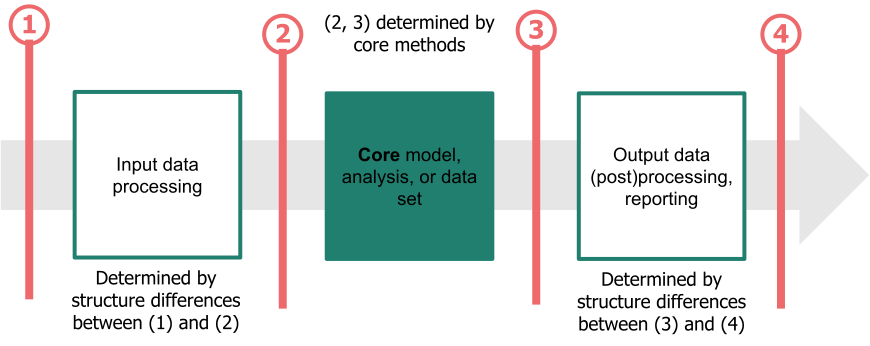
\includegraphics[width=\paperwidth]{data-stages.pdf}
\end{frame}

\section{(older slides)}

\includepdf[pages={10-12}]{../2021/12-01_IAMC.pdf}

\section{Planned improvements}

\subsection{Initial public release}

\begin{frame}
  \frametitle{Initial public release}

  Work beginning 2023-Q3, completing 2023-Q4.

  \bigskip
  Target:
  \begin{itemize}
    \item \texttt{message\_ix\_models.model.transport} —i.e. a module in the public MESSAGEix modeling tools repository, next to \texttt{.water} and others.
    \item Complete documentation \& test suite.
    \item Data prepped for R12 nodes, with clear declaration of data needs for application to other geographies.
  \end{itemize}
\end{frame}

\subsection{Shared \& autonomous LDV techs}
\subsection{Operational concept of ‘activity’}

% Planned improvements
\includepdf[pages={31-32}]{../2021/12-01_IAMC.pdf}

\section{Energy services in general}

\begin{frame}
  \frametitle{Energy services in general}

  \tableofcontents[currentsection]

\end{frame}

\subsection{MESSAGE/LP techniques for demand-side sectors}

\begin{frame}[allowframebreaks]
  \frametitle{LP techniques for demand-side sectors}

  \bigskip
  Original/natural mapping of the MESSAGEix \texttt{commodity}, and \texttt{technology} concepts:
  \begin{itemize}
    \item A measurable quantity of a physical object, e.g. \texttt{coal}.
    \item A artifact/machine that performs a physical process, e.g. \texttt{coal\_ppl}.
  \end{itemize}

  \bigskip
  \emph{Energy services} are often conceived as intangible (“health”, “access”), socio-cultural concepts measured as constructed quantities (“disability-adjusted life-year (DALY)” vs. “kg of coal”).

  \framebreak
  \structure{“Pseudo”}-technologies and commodities.
  \begin{itemize}
    \item Represent a quantity that is \emph{measurable} but perhaps not \emph{physical} as a “\texttt{commodity}”.
    \item Express MESSAGEix \texttt{demand} in these commodities.
    \item Represent a socio-technical process or relationship between two commodities (in the above sense) as a “\texttt{technology}”.
  \end{itemize}

  \bigskip
  MESSAGEix-Transport example:
  \begin{itemize}
    \item Transport activity various measures (distance traveled by a vehicle; distance traveled by a person; trips) → \texttt{commodity}
    \item “Usage” and “occupancy” of vehicles by people to obtain the energy service of passenger-distance traveled → \texttt{technology}.
  \end{itemize}

\end{frame}

\subsection{Systems theory for global modeling}

\begin{frame}[allowframebreaks]
  \frametitle{Systems theory for global modeling}

  In general, IAMs are always dependent on data and other models that treat the real-world phenomena in much greater detail, with domain-specific theory \& methods.

  \bigskip
  For example, in transport:
  \begin{itemize}
    \item Short-distance passenger: agent-based microsimulation of daily activity particular cities or model cities.
    \item Interaction of land-use, built environment, and mobility: “ILUTE”.
    \item Choice of vehicle technology or new modes (sharing, etc.):
    \item Aviation: models of airport expansion, new aircraft technologies.
    \item International freight: gravity models connecting ports.
  \end{itemize}

  \bigskip
  How do we preserve the information/validity of these while connecting or emulating them in IAMs?

  \bigskip
  → Recall and apply engineering systems theory.
\end{frame}

% Systems slides
\includepdf[pages={35-44}]{../2021/12-01_IAMC.pdf}

\begin{frame}[plain]

  \centering \Huge \structure{\bfseries Thank you!}

\end{frame}

\begin{frame}
  \frametitle{Contents}
  \tableofcontents
\end{frame}

% References
\includepdf[pages={28}]{../2021/12-01_IAMC.pdf}

\end{document}
